\documentclass[10pt]{article}
\usepackage[top=1.00in, bottom=1.0in, left=1in, right=1in]{geometry}
\renewcommand{\baselinestretch}{1.1}
\usepackage{graphicx}
\usepackage{natbib}
\usepackage{amsmath}
\usepackage{parskip}
\usepackage{wrapfigure}
\usepackage{multicol}


\def\labelitemi{--}
\parindent=0pt

\begin{document}

% To do! Add a full citation to Luke's book

\begin{multicols}{2}

\section*{A note on our notation}

\emph{Written by E. M. Wolkovich, with extensive help from T. J. Davies and V. Van der Meersch. Thanks also to Liam Revell for explaining basic BM notation.}

In the paper \citet{morales2024phylogenetic} we present a hierarchical phylogenetic model using a common but confusing notation for the parameterization of the species $\times$ species matrix. Here I try to clarify and correct the notation a little. 

The goal of the model is to understand how environmental cues (forcing, chilliing, photoperiod) affect budburst across species; I will just skip all this though and consider an intercept only model for simplicity. 

Let's speed through the start of the model as the notation there is unchanged. For each observation $i$ of species $j$, we assumed that the timing of phenological events were generated from the following sampling distribution:

\begin{align*}
  \label{modely}
  y_{i,j} \sim \mathcal{N}(\mu_j, \sigma_e^2)
\end{align*}
where
\begin{align*}
  \label{modelmu}
  \mu_j = \alpha_j 
  \end{align*}
and $\sigma_e^2$ represents random error unrelated to the phylogeny. And the species-specific intercept $\alpha_j$ is elements of the following normal random vectors:

\begin{align*}
    \label{phybetas}
  \boldsymbol{\alpha} = [\alpha_1, \ldots, \alpha_n]^T & \text{ such that }
  \boldsymbol{\alpha} \sim \mathcal{N}(\mu_{\alpha},\boldsymbol{\Sigma_{\alpha}}) 
\end{align*}

\noindent where the means of the multivariate normal distributions are root trait values (i.e., budburst date prior to evolving across a phylogenetic tree) and $\boldsymbol{\Sigma_{\alpha}}$ is an $n \times n$ phylogenetic variance-covariance matrix of the form ({\bf this is where it gets confusing}): \\ 
\begin{align*}
  \label{phymatold}
\begin{bmatrix}
  \sigma^2_i & \lambda_i \times \sigma_{i} \times \rho_{12} & \ldots & \lambda_i \times \sigma_{i} \times \rho_{1n} \\
  \lambda_i \times \sigma_i \times \rho_{21} & \sigma^2_i & \ldots & \lambda_i \times \sigma_{i} \times \rho_{2n} \\
  \vdots & \vdots & \ddots & \vdots \\
  \lambda_i \times \sigma_i \times \rho_{n1} & \lambda_i \times \sigma_i \times \rho_{n2} & \ldots & \sigma^2_i \\
\end{bmatrix}
\end{align*}

\noindent where $\sigma_i^2$ is the rate of evolution across a tree for a given trait or predictor (here assumed to be constant along all branches), $\lambda_i$ scales branch lengths and therefore is a measure of the phylogenetic signal or extent of phylogenetic relatedness on each model parameter (i.e., $\alpha_{j}$), and $\rho_{xy}$ is the phylogenetic correlation between species $x$ and $y$, or the fraction of the tree shared by the two species.

{\bf What's confusing here?} 

A few things. First, the $i$ notation mixed with the numbers on $\rho_{xy}$ is not really helpful, and it's made worse by our choice to use both $\sigma^2$ and $\sigma$ notation here (and you may now notice---we never defined those  $\sigma$). Here $\sigma^2$ is the Brownian motion rate of evolution across the tree, and the other $\sigma$ should also be squared (see below `Want even more information?' for more details). So the above works if you drop the $i$ notation (it never should have been on  $\sigma^2$ or $\lambda$ in my estimation as these are single parameters estimated across the entire tree) and square all the $\sigma$ as shown below:

\begin{align*}
  \label{phymatnew}
\begin{bmatrix}
  \sigma^2 & \lambda \times \sigma^2 \times \rho_{12} & \ldots & \lambda \times \sigma^2 \times \rho_{1n} \\
  \lambda \times \sigma^2 \times \rho_{21} & \sigma^2 & \ldots & \lambda \times \sigma^2 \times \rho_{2n} \\
  \vdots & \vdots & \ddots & \vdots \\
  \lambda \times \sigma^2 \times \rho_{n1} & \lambda \times \sigma^2 \times \rho_{n2} & \ldots & \sigma^2\\
\end{bmatrix}
\end{align*}

%%
We could have also correctly written this as:

\begin{align*}
  \label{phymatalt}
\begin{bmatrix}
  \sigma^2 & \lambda \times \sigma_{12} & \ldots & \lambda \times \sigma_{1n} \\
  \lambda \times \sigma_{21} & \sigma^2 & \ldots & \lambda \times \sigma_{2n} \\
  \vdots & \vdots & \ddots & \vdots \\
  \lambda \times \sigma_{n1} & \lambda \times \sigma_{n2} & \ldots & \sigma^2 \\
\end{bmatrix}
\end{align*}

Above I have dropped $\rho$ (it's just inherently in there, apparently this is a thing people do). Now $\sigma^2$ is still the Brownian motion rate of evolution across the tree, and $\sigma$ is the covariance between representative taxa. This is not an uncommon representation but I think we could have been clearer if we presented the last part of our notation as:

\added{
  \label{phymatbest}
  \begin{equation} {\bf \Sigma_{\alpha}}  =  \sigma^2_{BM} \cdot 
\begin{bmatrix}
  \rho_{1,1} & \lambda \cdot \rho_{1,2} & \ldots & \lambda \cdot \rho_{1,n} \\
  \lambda \cdot \rho_{2,1} &  \rho_{2,2} & \ldots & \lambda \cdot \rho_{2,n} \\
  \vdots & \vdots & \ddots & \vdots \\
  \lambda \cdot \rho_{n,1} & \lambda \cdot \rho_{n,2} & \ldots & \rho_{n,n}\\
\end{bmatrix}
}

Here I moved $ \sigma^2$ to outside the matrix since it a common factor multiplied across elements of the matrix (and I added  $_{BM}$ to denote Brownian Motion). Then I show the $\rho$ across all elements also, even the diagonals (and I use the dot multiplier throughout, and I add a common in the subscript when referencing elements, both of which I find easier to read). 

At this point, I will add that $\lambda$ is a multiplier of the off-diagonal elements (as you can see), where estimates of $\lambda = 1$ essentially leave the matrix untransformed and suggest that the species intercepts (or $\beta$ etc.) are completely consistent with Brownian motion, while estimates of $\lambda = 0$ suggest no phylogenetic patterning according to Brownian motion. Further, when $\lambda = 0$ the model effectively defaults to a normal distribution, and thus simple partial pooling (or `random effects' if you really want to call it that). 

\section*{Want even more information?}

You can also check out  \cite{pearse2025define}, where we tried to do the notation much better in explaining this for variance-covariance matrices. If you want even more, I have included below a basically verbatim version of information kindly sent from Liam Revell:

First, this is from Chapter 3 of Luke's book.

\setlength{\intextsep}{6pt} 
\begin{wrapfigure}
\centering
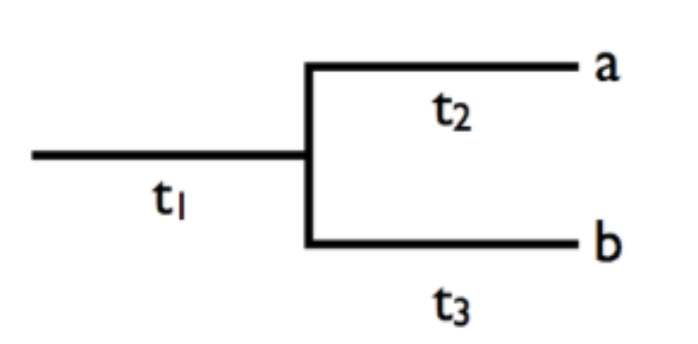
\includegraphics[width=0.41\textwidth]{figs/revellemail1.png} 
 %  \caption{A tree, from \emph{Phylogenetic Comparative Methods}} 
  \label{fig:tree}
\end{wrapfigure}

Here the variance of taxon a might be denoted $\sigma(a)^2$ and under our Brownian process the value of $\sigma(a)^2$ would be $\sigma(B)^2 * (t1 + t2)$ in which $\sigma(B)^2$ is the Brownian rate. (It's given using the symbol for a variance because it's specifically the rate at which variance accumulates under our stochastic process.) The covariance between taxa a and b we might give as $\sigma(a,b)$ and in this case it'll have a value of $\sigma(B)^2 * t1$ -- the rate of evolution multiplied by the evolutionary history shared between the two taxa, a and b.

If we jump to Chapter 6 of Luke's book then we see:

\setlength{\intextsep}{6pt} 
\begin{wrapfigure}
\centering
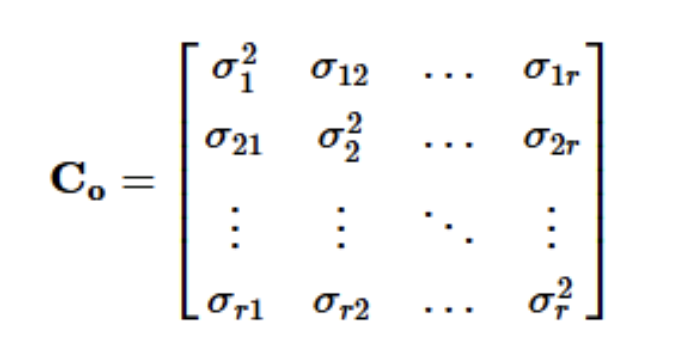
\includegraphics[width=0.41\textwidth]{figs/revellemail2.png} 
 %  \caption{A tree, from \emph{Phylogenetic Comparative Methods}} 
  \label{fig:c0}
\end{wrapfigure}

This is just the covariance matrix... so $\sigma(1)^2$ is the variance for taxon 1, which we'd calculate under Brownian motion as $\sigma(B)^2$ time the sum of the edge lengths leading from the root of the tree to the taxon 1 (or equivalently, the height above the root of taxon 1); $\sigma(12)$ is the covariance of taxa 1 and 2 which we'd calculate as \$sigma(B)^2$ times the height above the root of the MRCA (most recent common ancestor) of taxa 1 and 2; and so on.

When introducing lambda, we can think of it as a transformation of the covariance matrix in which all non- diagonal elements are multiplied by lambda.

\setlength{\intextsep}{6pt} 
\begin{wrapfigure}
\centering
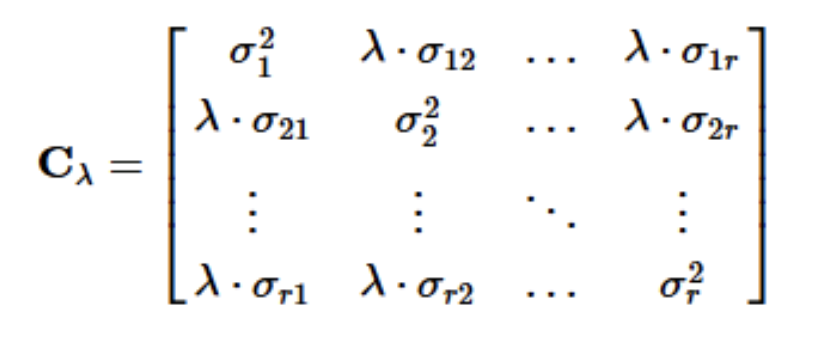
\includegraphics[width=0.41\textwidth]{figs/revellemail3.png} 
 %  \caption{A tree, from \emph{Phylogenetic Comparative Methods}} 
  \label{fig:clambda}
\end{wrapfigure}

However, since $\sigma(B)^2$ (the rate of Brownian evolution) is a common factor of all the elements in $C$, we could equivalently first factor out $\sigma(B)^2$, and then multiply what's left (the times above the root of the MRCA of each $_{i,jth}$ pair of taxa) by $\lambda$. The result is the same. (This is why lambda is sometimes also represented as a tree transformation.)

\bibliographystyle{refs/iambeststyle}
\bibliography{refs/fixnotationmc2024}


\end{document}
